\section{Theoretischer Hintergrund}

\subsection{Allgemeine Definitionen}

\paragraph{Elektrische Flexibilität:}

% s. Anyas Folien vom Workshop - räumlich und zeitlich

\paragraph{Netzebenen:}

Das Stromnetz lässt sich grundsätzlich in Übertragungs- und Verteilnetze unterteilen.
Das Übertragungsnetz dient dem Transport von Strom über lange Strecken bei hohen Spannungen.
Ergänzend erfolgt in den Verteilnetzen die regionale Feinverteilung bei geringeren Spannungen. \cite{Agora2019}\medskip

Innerhalb der Verteilnetze wird zwischen drei Spannungsebenen unterschieden. Hierzu zählen die \glspl{HS}-, \glspl{MS}- und \glspl{NS}-Ebene.
In \autoref{tab:Spannungsebenen} finden sich die üblichen Spannungen je Spannungsebene und die verbaute Stromkreislänge in Deutschland je Spannungsebene.
Innerhalb dieser Masterarbeit werden ausschließlich die Effekte auf die Verteilnetze auf \glspl{MS}- und \glspl{NS}-Ebene untersucht.

{
\renewcommand{\arraystretch}{1.2}% grßerer Zeilenabstand
\sisetup{range-phrase=~bis~}
\begin{table}[H]
	\begin{center}
		\caption{Übliche Spannung und Stromkreislänge der Spannungsebenen im deutschen Verteilnetz}
		\begin{tabu} to 0.65\textwidth {X[0.75] X[1, r] X[1, r]}
			\toprule
            Spannungsebene & Spannung               	& Stromkreislänge   \\\midrule
            Hochspannung   & \SIrange{60}{110}{\kv}     & \SI{95000}{\km}   \\
            Mittelspannung & \SIrange{6}{30}{\kv}  		& \SI{510000}{\km}  \\
            Niederspannung & \SI{230}{\V} 				& \SI{1100000}{\km} \\\bottomrule
            \multicolumn{3}{l}{Quellen: \cite{BDEW2016} und \cite{BMWiNetz}}
		\end{tabu}
		\label{tab:Spannungsebenen}
	\end{center}
	\vspace{-3mm}%Put here to reduce too much white space after your table
\end{table}
}


\paragraph{Netztopologie:}

\gls{NS}-Netze werden in dieser Arbeit ausschließlich als Strahlennetze ausgelegt.
Strahlennetze werden so genannt, weil die einzelnen Stränge der Netze strahlenförmig vom Ortsnetztransformator zu den Endverbrauchern verlaufen. \cite{Agora2019}
Vorteil dieser Form von Netzen ist die leichte Berechenbarkeit und die einfache Überwachung des Netzzustandes.
Jedoch führt bereits ein einziger Fehlerfall an einer Einspeisestelle eines Verbrauchers dazu, dass das auch alle nachfolgenden Verbraucher vom Netz getrennt sind.
Auch nimmt der Spannungsabfall über die Länge der Leitung immer weiter zu, was zu einer geringeren Belastbarkeit am Ende der Leitung führt. \cite{WNG2020}\medskip

Im Gegensatz dazu werden \gls{MS}-Netze als Ringnetze betrieben.
Ringnetze bieten den Vorteil, dass diese von zwei Seiten gespeist werden, wodurch ein Ringform entsteht.
Hierdurch können im Falle einer Störung weiterhin alle anderen Verbraucher versorgt werden.
Jedoch werden diese Ringnetze in der Regel offen betrieben.
Dies bedeutet, dass sich etwa in der Mitte des Rings eine offene Trennstelle befindet.
Auf diese Weise können Ringnetze ebenso einfach überwacht werden wie Strahlennetze.
Im Fehlerfall wird bei dieser Baumform maximal ungefähr die Hälfte der Verbraucher vom Netz getrennt.
Durch das Schließen der Trennstelle können dann wieder alle Verbraucher, mit Ausnahme des Fehlerfalls, versorgt werden. \cite{WNG2020} \cite{Westermann2019}

\paragraph{Gleichzeitigkeit:}

\subsection{Elektromobilität}

\paragraph{Ladestrategien:}

Der Ladevorgang von \glspl{EV} kann durch unterschiedliche äußere Anreize gesteuert werden. Grundsätzlich lassen sich hierbei marktorientierte und netzdienliche Ladestrategien unterscheiden.


\subparagraph{Marktorientierte Ladestrategien} haben als Fokus die Minimierung der Kosten für den Strombezug. Dies bedeutet konkret, dass die Ladevorgänge durch ein Preissignal am Großhandelsmarkt ausgelöst beziehungsweise unterbrochen werden. Eine solche Ladestrategie kann sowohl positive als auch negative Effekte aufweisen und erfordern einen geeigneten rechtlichen Rahmen. So führt beispielsweise ein hohes Stromangebot zu niedrigen Großhandelsmarktpreisen, wodurch das beladen der \glspl{EV} ausgelöst wird und ein Ausgleich zwischen Angebot und Nachfrage angestrebt wird. Auf der anderen Seite werden lokale Netzengpässe nicht berücksichtigt und die Gleichzeitigkeit der Ladevorgänge erhöht sich, wodurch sich der Netzausbaubedarf erhöhen kann. \cite{Agora2019} \cite{Dorendorf2019}

% BW Verteilnetzstudie: Bei einem marktorientierten Betrieb von Flexibilitätsoptionen richten sich diese in ihrem Betriebsverhalten nach den Anforderungen eines überregionalen Marktes.
% Als Ergebnis des Analyseschrittes ist bekannt, welches Betriebsverhalten die betrachteten Flexibilitätsoptionen bei einer marktorientierten Nutzung aufweisen können. Hierbei zeigt sich, dass die überregionalen Flexibilitätssignale eine hohe Gleichzeitigkeit im Betrieb insbesondere der lastseitigen Flexibilitätsoptionen auslösen. Besonders bei EV findet eine starke Konzentration der Ladevorgänge auf die frühen Morgenstunden statt (siehe Abbildung 6.6). 


\subparagraph{Netzdienliche Ladestrategien} setzen hingegen auf die Vermeidung von lokalen Engpässen, welche durch eine hohe Nachfrage entstehen können. Hierbei kann zwischen präventiven und kurative Maßnahmen unterschieden werden. Präventive Maßnahmen sollen Kunden dazu bewegen, ihre Ladevorgänge in Zeiten geringer Netzauslastung zu verlegen. Dies kann zum Beispiel über monetäre Anreize aber auch über Quoten erfolgen. Bei kurativen Maßnahmen handelt es sich hingegen um ein aktives Eingreifen durch den Netzbetreiber, welcher bei drohenden Netzengpässen in den Ladevorgang eingreift. \cite{Agora2019}


\subsection{ding0}\label{chap:dingo_theo}

Eine der Grundlagen für die Nutzung des Netzplanungsinstruments \edisgodot, sind die zu untersuchenden Netztopologien der \gls{MS}- und \gls{NS}-Ebene.
Aufgrund der mangelnden Datenlagen von reale Netztopologien werden, wird auf synthetisch erzeugte Netztopologien zurückgegriffen.
die mit Hilfe des Software Tools \dingo erzeugt wurden.
Das Tool ist in der Lage ländliche und suburbane Netzstrukturen zu synthetisieren und kann auf GitHub \cite{dingo2019} öffentlich eingesehen und frei verwendet werden.
Weiterhin findet sich auf ReadTheDocs \cite{dingo-docs2019} eine ausführliche Dokumentation.
Die Synthetisierung der Netztopologien ist nicht Teil dieser Masterarbeit und erfolgte innerhalb des \openego Projektes. \cite{Mueller2019} Die Netztopologien entsprechen dem Stand von \num{2015}.


\paragraph{Mittelspannung}

Auf der \gls{MS}-Ebene gibt es \num{3591} Netzgebiete mit einer mittleren Fläche von \SI{99}{\km\squared}.
Die einzelnen \gls{MS}-Netze werden alle als offene Ringnetze betrieben.
Im städtischen Bereich werden hauptsächlich Erdkabel mit einer Nennspannung von \SI{10}{\kv} eingesetzt, während im ländlichen Raum größtenteils Freileitungen mit einer Nennspannung von \SI{20}{\kv} eingesetzt werden. \cite{Mueller2019}


\paragraph{Niederspannung}

Die \gls{NS}-Ebene wird mit Hilfe von \num{46} Referenznetzsträngen synthetisiert.
Die Referenznetzsträngen stehen repräsentativ für eine bestimmte Anzahl an Hausanschlüssen und werden jeweils einer Netzklasse zugeordnet.
Hierbei wird auf Grundlage der Anzahl an Hausanschlüssen je Ortsnetzstation zwischen Land-, Dorf- und Vorstadtnetzen unterschieden.
Die verschiedenen Referenznetzstränge werden so miteinander kombiniert, dass für eine bestimmte Zahl an Hausanschlüssen innerhalb einer Netzklasse ein typisches Netz generiert wird. \cite{Mueller2019}


\subsection{K-Means-Clustering}

Die große Anzahl an Netzgebieten und die hohe räumliche und zeitliche Auflösung des Netzdatenmodells führen zu inakzeptabel hohen Rechenzeiten.
Um die Komplexität des Modells zu reduzieren, werden mit Hilfe des \kmeans Referenznetzgebiete ausgewählt, die stellvertretend für eine möglichst große Zahl an Netzgebieten stehen.
Das \kmeans wurde im Rahmen des \openego Projektes entwickelt und wird in dieser Arbeit unverändert angewendet. \cite{Mueller2019}\medskip

Grundlage des \kmeans bildet der \texttt{expectation–maximization-Algorithmus} (EM-Algorithmus) des Python Paketes \texttt{scikit learn}. \cite{scikit-learn2011}
Der Algorithmus bildet durch die Minimierung der Summe der quadrierten gewichteten euklidischen Abstände zwischen den originalen Netzknoten und den Clusterzentren eine gewollte Anzahl \texttt{k} an Clustern.
Die Gewichtung erfolgt hierbei anhand der angeschlossenen konventionellen und des angeschlossenen Verbrauchs am Netzknoten.
Dabei werden folgende Schritte durch den Algorithmus durchlaufen:

\begin{enumerate}
	\item Zufällige Auswahl von Clusterzentren
	\item E-Step: Alle Netzknoten dem nächstgelegenen Clusterzentrum zuweisen
	\item M-Step: Neues Clusterzentrum auf den Schwerpunkt der zugewiesenen Netzknoten setzen
	\item Die Schritte E und M werden so lange wiederholt, bis Konvergenz auftritt
\end{enumerate}

% TODO: enumerate ist komplett abgeschrieben. anders zitieren?
% TODO: Grafik 5.3 aus open_ego Bericht einfügen

In {\color{red} TODO} findet sich eine exemplarische Darstellung des EM-Algorithmus.
In dieser Arbeit wird stellvertretend für das Cluster, dass Netzgebiet mit dem minimalen quadrierten gewichteten euklidischen Abstand zum Clusterzentrum verwendet.


\subsection{simBEV}\label{chap:simbev_theo}

% TODO: pro­ba­bi­lis­tischen Ansatz mathematisch erklären

Mit Hilfe des im Rahmen dieser Masterarbeit mitentwickelten Software Tools \simbev können die Fahrtprofile für eine beliebige Anzahl an Fahrzeugen verschiedener Fahrzeugklassen erstellt werden.
Weiterhin kann hierbei zwischen den in \autoref{tab:RegioStaR} aufgelisteten \Regiostar Raumtypen unterschieden werden, um das raumtypenspezifische Fahrverhalten abzubilden.

{
\renewcommand{\arraystretch}{1.2}% grßerer Zeilenabstand
\sisetup{range-phrase=~oder~}
\begin{table}[H]
	\begin{center}
		\caption{Regionalstatischer Raumtypen (RegioStaR 7)}
		\begin{tabu} to \textwidth {X[1] X[2]}
			\hline
			Raumtyp Nummer & Regionalstatischer Raumtyp                                \\ \hline
			\num{71}       & Metropolen                                                \\
			\num{72}       & Regiopolen und Großstädte                                 \\
			\num{73}       & Mittelstädte, städtischer Raum einer Stadtregion          \\
			\num{74}       & Kleinstädtischer dörflicher Raum einer Stadtregion        \\
			\num{75}       & Zentrale Städte einer Ländlichen Region                   \\
			\num{76}       & Mittelstädte, städtischer Raum                            \\
			\num{77}       & Kleinstädtischer, dörflicher Raum einer Ländlichen Region \\ \hline
            \multicolumn{2}{l}{Quelle: \cite{BMVI2020}}
		\end{tabu}
		\label{tab:RegioStaR}
	\end{center}
	\vspace{-3mm}%Put here to reduce too much white space after your table
\end{table}
}

Die Fahrtprofile werden über einen pro­ba­bi­lis­tischen Ansatz auf Grundlage der Befragung \gls{MID} \cite{ISGH2017} erstellt.
Dabei erhält jeder simulierte Zeitschritt eine Wahrscheinlichkeit für einen bestimmten Wegezweck eine Fahrt zu beginnen.
Löst ein Fahrzeug eine Fahrt aus, wird abhängig vom Wegezweck und Regionstyp der Fahrt, ebenfalls pro­ba­bi­lis­tisch, eine Streckenlänge und eine anschließende Standzeit zugeteilt.
Der hierbei entstehende Verbrauch des Fahrzeuges muss anschließend gedeckt werden.
Ob am Zielort ein Ladevorgang stattfindet, hängt vom \gls{SOC} des Fahrzeuges und dem Vorhandensein eines Ladepunktes ab.
Ob ein Ladepunkt am Zielort zur Verfügung steht und welche Ladeleistung dieser aufweist, wird mit Hilfe der Wahrscheinlichkeiten aus \autoref{tab:WegezweckProbability2050} ermittelt.
Ladepunkte besitzen pauschal einen Wirkungsgrad von \SI{90}{\percent}. % TODO: Quelle
Die Bestimmung des Vorhandenseins eines Ladepunktes zu Hause und am Arbeitsplatz erfolgt je \gls{EPKW} einmalig und wird anschließend konstant gehalten.
Für alle anderen Wegezwecke, erfolgt die Bestimmung kontinuierlich.
Wurde dem Zielort ein Ladepunkt zugeordnet wird davon ausgegangen, dass der Fahrzeugnutzer einen Ladevorgang erst ab einem bestimmten \gls{SOC} einleitet, da dies einen zusätzlichen Aufwand für den Nutzer bedeutet.
Dabei wird angenommen, dass das Laden des Fahrzeuges am Wohnort und am Arbeitsplatz bereits ab einem \gls{SOC} von \SI{95}{\percent} stattfindet.
Im öffentlichen Raum bedeutet das Anfahren und der Anschluss an einen Ladepunkt einen größeren Aufwand für den Nutzer als im privaten Raum.
Deshalb wird angenommen, dass oberhalb eines \glspl{SOC} von \SI{80}{\percent} keine Ladevorgänge stattfinden.
Es gilt je niedriger der \gls{SOC}, desto wahrscheinlicher ist es, dass die öffentliche Ladeinfrastruktur genutzt wird.
Ab einem \gls{SOC} von \SI{50}{\percent} findet, wann immer möglich, eine Ladung des Fahrzeugs statt.
Zwischen den beiden Stützwerten erfolgt eine lineare Interpolation, welche in \autoref{fig:soc_charging_prob} visualisiert wurde.

\begin{figure}[H]
    \centering
    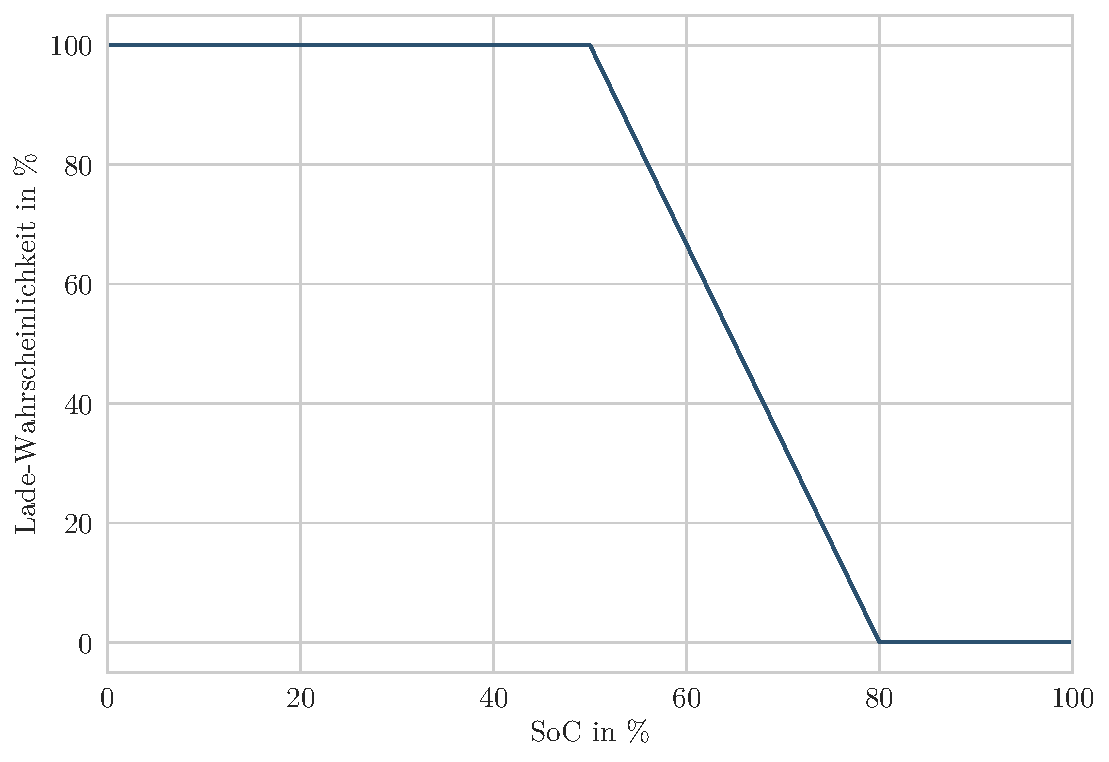
\includegraphics[width=\textwidth]{Bilder/soc_charging_prob}
    \caption{Abhängigkeit der Ladewahrscheinlichkeit vom SoC an öffentlichen Standorten}\label{fig:soc_charging_prob}
\end{figure}

Schnellladeinfrastruktur besitzt aufgrund des zusätzlichen Fahrt- und Zeitaufwandes eine geringe Attraktivität für den Nutzer.
Deshalb wird eine Schnellladung in dieser Simulation nur dann ausgelöst, wenn es wirklich nötig ist.
Sinkt der \gls{SOC} eines Fahrzeugs unter \SI{20}{\percent}, wird eine Schnellladestation angefahren und das Fahrzeug wird für \SI{15}{\Minuten} geladen.
Im Unterschied zu \glspl{BEV}, können \glspl{PHEV} auch mit einem \gls{SOC} von \SI{0}{\percent} ihre Fahrt mit Hilfe des Verbrennungsmotors fortsetzen.
Aus diesem Grund wird bei \glspl{PHEV} kein Schnellladevorgang ausgelöst.


\subsection{eDisGo}\label{chap:edisgo_theo}

\paragraph{Netzausbaubedarf:}

% s. Verteilnetzstudie BW
% Die festgestellten Grenzwertverletzungen werden wie folgt priorisiert:
% 1. Verletzung der thermischen Transformatorbetriebsgrenzen
% 2. Verletzungen des Spannungsbandes
% 3. Verletzung der thermischen Leitungsbetriebsgrenzen

\subparagraph{Minimaler Residuallastfall und Maximaler Residuallastfall}

\subparagraph{Thermischen Betriebsmittelbelastung}

\subparagraph{Maximale Knotenspannungen}

% Spannungsband

\subparagraph{n-1}

\paragraph{Netzausbaumaßnahmen:}

% BW: In der klassischen Netzplanung erfolgt die Bestimmung der auslegungsrelevanten Betriebsfälle anhand der installierten Leistung einzelner Verbraucher, gemessenen Spitzenlasten oder auf Basis von Erfahrungswerten bezüglich der Gleichzeitigkeit bestimmter Verbraucher. Eine Netzplanung auf Basis von Zeitreihen findet in Verteilnetzen in der Regel nicht statt. Da die Analyse des Betriebsverhaltens von Flexibilitätsoptionen jedoch auf der Betrachtung von Zeitreihen aufbaut, ergibt sich das Problem der Übertragbarkeit von Erkenntnissen aus der Zeitreihenanalyse auf die Netzplanung.

\subparagraph{rONT}

% Ergebnis Workshop: i.d.R. zu teuer und unnötig

% BW: Eine häufige Ursache für Netzausbaubedarf bzw. auftretende restriktive Randbedingung für die Integration von DEA in NS-Netze ist die Einhaltung der Spannungsqualität beim Verbraucher gemäß DIN EN 50160 [16]. 

\subparagraph{Spannungsbandaufteilung}

\subparagraph{Optimierte Einstellung eines lastfrei stufbaren Transformators}